\documentclass[11pt]{article}
\usepackage{common}
\usepackage[utf8]{inputenc}

\title{Presidents Game Playing Agent}
\author{Nicholas Larus-Stone \and Juan Perdomo \and Matt Goldberg}

\pagenumbering{arabic}

\begin{document}
\maketitle{}

\section{Introduction}

This paper provides an in-depth investigation of a number of algorithms applied to the multiplayer card game Presidents. The overarching goal of this investigation is to develop an agent that can intelligently play the game and compete against skillful human opponents.   Presidents presents an interesting problem because it is a game involving imperfect information, making it much more difficult to choose an optimal strategy. We first applied two common multiplayer game playing algorithms to this problem: paranoid and max-n \cite{sturtevant03a}. Neither algorithm inherently handles uncertainty, so we had to develop our own methods for dealing with imperfect information. We also investigated more complex algorithms that are better at handling uncertainty: Monte Carlo Tree Search \cite{browne12} and reinforcement learning \cite{fujita03}. Our objective was to apply all of these algorithms to Presidents and determine which one offered us the best performance.\\

The algorithms we implemented were largely derived from the minimax algorithm we talked about in class. However, due to the increased complexity of Presidents, we also had to innovate in order to deal with the imperfect information--for this we drew inspiration from our unit on inference and uncertainty. We will first describe how each of the algorithms were implemented, then we will discuss their results and analyze the effectiveness of our implementations to this specific problem. Finally, we will point out some of the areas for further research that our work led us towards.

\section{Background}

Research into game playing has been a main focus of members of the artificial intelligence community since the mid 20th century. As mentioned in lecture by Prof. Rush, computer scientists worked on topics such as chess AI as early as 1959 \footnote{Rush, Adversarial Search and Games}. Although research into game playing algorithms might seem like an inefficient investment of resources by talented researchers, breakthroughs in the algorithms and techniques designed for  simple games such as chess or Go have often had repercussions in other fields that have more of a direct impact on society. At their essence, these algorithms work to find solutions to problems in which players compete to maximize their rewards under certain constraints. In the case of Presidents, however, there is the additional complication of having imperfect information as each individual agent must operate without knowing the hands of his opponents. Developments in game playing algorithms for problems like Presidents therefore can provide insights into different real life problems such as auctions in which a number of agents compete to achieve certain goals using incomplete information.\\


The first two algorithms discussed in this paper, paranoid and max$^n$ are essentially extensions of the traditional MiniMax algorithm developed by John von Neumann in 1928 \footnote{Kjeldsen, John von Neumann's Conception of the Minimax Theorem: A Journey Through Different Mathematical Contexts}. Since its origins, however, several optimizations have been introduced such as the use of Alpha Beta Pruning to reduce the size of the search space and techniques to deal with imperfect information. Moreover, research into techniques to deal with uncertainty has become a hall mark of 21st century computer science and artificial intelligence. Conversely to Paranoid and Minimax, Monte Carlo Tree Search has been developed more recently, first appearing in a paper by Remi Coulomb in 2006. Although Monte Carlo methods have their origins in the 1940s and the Manhattan Project, the creation of the MCTS algorithm for games is a 21st century discovery.



\subsection{Rules of Presidents}

The rules of the game are simple. The deck is dealt out evenly to all players. The goal of the game is to get rid out of all your cards as quickly as possible. In order to do so, you can only play cards higher than the current card at the top of the stack. 3's are the lowest cards and 2's are the highest. Once a 2 has been played, the stack is cleared and the player who played it gets to go again. There are a few extra rules. Order of play is decided by the player who has the 3 of clubs and then others play clockwise in the order they are seated. If the stack is clear, a player can choose to play doubles or triples and the players following him must also play higher doubles or triples. A player can choose to pass at any point in the game even if he has legal actions in that state. Lastly, after the game is done, the first two players to finish become President and Vice President and the last two become Asshole and Vice Asshole. For the following round of play, the President has the right to the Assholes' 2 best cards and the VP takes the VA's best card while at the same time handing them back a card of their choice (usually their lowest). The rest of the players don't switch any of their cards.

\section{Related Work}

During our research into game playing methods for Presidents. We found no algorithms that dealt specifically with the game of presidents, however, we did find research in related fields such as card playing AI agents and agents for games of incomplete information, the most common of which was the popular card game Hearts.  Multiplayer Games, Algorithms and Approaches by Sturtevant was was particularly helpful to learn about extensions of Minimax to multi agent games \cite{sturtevant03b}. Koller's work on imperfect information provided insights into adaptations of traditional game playing agents for scenarios in which there is imperfect information\cite{pfeffer95}. Lastly, papers by Sturtevant and Browne on Max-N, Paranoid, and Monte Carlo Tree Search methods served as guides that led our initial development of the algorithms used\cite{sturtevant03a, browne12}.



\section{Overview of Algorithms}

\subsection{Paranoid}

The first algorithm we implemented was a paranoid agent. The paranoid algorithm is a modified minimax algorithm which assumes that all the other players in the game are collaborating against it. It does this at the evaluation step, by estimating values for each of the players, then returning the max player's value minus the sum of the other players' values. This reduces the multiplayer game to a two player one in which traditional minimax can be applied.

The tricky part is that the game tree is so large that it's impossible to expand out the tree fully. So, we had a cutoff point for our algorithm to stop evaluating (usually 2 rounds of play). However, this means that we didn't have access to the results of the game, only what we thought the game looked like. This meant we had to use a heuristic to evaluate how good the state was for us. As we will talk about later, creating a heuristic for this game is quite difficult, but also incredibly important for the performance of these algorithms.

\begin{algorithm}
  \begin{algorithmic}
    \Procedure{Paranoid}{state, depth, player}
	\If{isTerminal(state) or depth $>$ MAXDEPTH}
		\State{values = evaluate(state)}
		\State{return values[0] - sum(values[1:])}
	\EndIf
	\If{isMax(player)}
		\State{v = -$\infty$}
	 	\For{action in LegalActions}
	 		\State{nextState = getNextState(state, action)}
			\State{v = max(v, paranoid(nextState, depth + 1, nextPlayer))}
			\State{a = action if v changed}
		\EndFor
	\EndIf
	\If{isMin(player)}
		\State{v = $\infty$}
	 	\For{action in LegalActions}
	 		\State{nextState = getNextState(state, action)}
			\State{v = min(v, paranoid(nextState, depth + 1, nextPlayer))}
			\State{a = action if v changed}
		\EndFor
	\EndIf
	\State{return a, v}
    \EndProcedure{}
  \end{algorithmic}
  \caption{Pseudocode for Paranoid Algorithm}
\end{algorithm}

\subsubsection{Pruning}

Something that is very nice about the paranoid algorithm is that since it is so closely related to minimax, $\alpha\beta$ pruning can be built on top of it. After the paranoid evaluation, we return an action and an associated value. This means we can keep track of what we would return from the current node and prune other sibling nodes if they would ever return a value that would not replace our value. When we implemented pruning, we saw a decrease in the number of nodes expanded by the Paranoid algorithm by about 500 nodes on average. Since the Paranoid algorithm expands about 3000 nodes when MAXDEPTH is two rounds, this was a dramatic increase in speed.

\subsection{Max$^n$}

The second algorithm we implemented was max$^n$. This algorithm adapts minimax to many players by having each player pick the action that maximizes the value to herself in the subsequent state. Values for states are represented by $n$-length tuples, where $n$ is the number of players, and where the $i$th entry in the tuple is the value of that state to player $i$. By contrast, when expanding the game tree in minimax, player 1 assumes the player 2 is minimizing player 1's value of the subsequent state; thus, in max$^n$, there is no ``Min'' agent, and instead every agent is a ``Max'' agent for their own value in the tuple.

Similarly to paranoid, the game tree is far too large to search to exhaustion, so the values are determined by a heuristic similarly. The values of child states are determined as follows: if the search depth exceeds a predefined maximum depth (we found 2 rounds of play to be a good tradeoff between search depth and speed), then the values are determined by a heuristic; if the search expands a tree to a terminal state, then the values are determined by where each player finishes in the game (i.e., coming in first and winning the presidency is better than coming in second and winning the vice presidency).

\begin{algorithm}
  \begin{algorithmic}
    \Procedure{MaxN}{state, depth, player}
    \If{isTerminal(state)}
      \State{values = evaluate(state)}
      \State \Return PASS, values
    \EndIf
    \If{depth $\geq$ MAXDEPTH}
      \State{bestAction = PASS}
      \State{bestVal = evaluate(state)}
      \State{actions = actions(player, state)}
      \ForAll{action in actions}
      \State{child = getChild(state, action)}
      \State{childVal = evaluate(child)}
	\If{childVal[player] $>$ bestVal[player]}
	  \State{bestAction = action}
	  \State{bestVal = childVal}
	\EndIf
      \EndFor
      \State{\Return bestAction, bestVal}
    \EndIf
    \State{bestAction = PASS}
    \State{bestVal = ($-\infty, \dots, -\infty$)}
    \State{actions = actions(player, state)}
    \ForAll{action in actions}
    \State{child = getChild(state, action)}
    \State{childAction, childVal = MaxN(child, depth $+1$, next(player))}
    \If{childVal[player] $>$ bestVal[player]}
      \State{bestAction = action}
      \State{bestVal = childVal}
    \EndIf
    \EndFor
    \State{\Return bestAction, bestVal}
\EndProcedure
  \end{algorithmic}
  \caption{Pseudocode for Max$^n$ Algorithm}
\end{algorithm}


\subsection{Monte Carlo Tree Search}

The MCTS algorithm is divided into 4 key stages: selection, expansion, simulation, and backpropagation. In selection, a node is chosen starting from the root of the game tree by recursively selecting the most promising child node until a leaf in the tree is reached. After a node has been chosen, the game is played out using a default policy until a result is reached. Lastly, in backpropagation, the result of the playout is incorporated recursively into each node located in the path from the root to the selected child.\\

\begin{algorithm}
  \begin{algorithmic}
    \Procedure{MCTS}{state}
	\State{root $\gets$ mctsNode(state)}
	\While{budget}
	 \State{nextNode $\gets$ selection(root)}
	 \State{result $\gets$ simulation(nextNode)}
	\State{backpropagate(nextNode, result)}
	\EndWhile{}
   \State{action $\gets$ bestChild(root)}
\State{return action}
    \EndProcedure{MCTS}
  \end{algorithmic}
  \caption{Pseudocode for Monte Carlo Tree Search}
\end{algorithm}

In the context of Presidents, a separate tree data structure to the state formalism had to be developed in order to implement MCTS. Each node in the tree contained variables describing the number of times each node had been visited as well as the score of the node. Moreover, each node contained a list of hands for each player and the id of the player whose turn it was to play. Since the hands of the other players in the game are unknown, when instantiating the tree, hands had to be sampled for the other agents in the game based on the sizes of each player's hand and the set of cards yet to be played. Each child node corresponded to the actions the player whose turn it was could make based on his hand and the top card on the deck. Scores were defined as the finishing position of the agent in the game. Since higher scores are better, we took the inverse of the finishing rank to indicate the score. \\

In the selection stage, we used the UCT algorithm developed by Kocsis and Szepesvari discussed by Browne in his paper on MCTS methods. It takes into account exploration and exploitation of paths down the tree by weighing the score of each node and the number of times it and its parent had been visited. Once a node is selected, the tree is expanded to include the children of that node and one of the child nodes is selected at random. In simulation, a game was played out based one the hands of each player at that node. Finally, in the backpropagragation stage the normalized score (raw score divided by number of visits) is sent up the tree to the node updating the values of each node along the way. This is run until a predetermined budget is used up, which in this case, we chose to be time. After the time ran out, the agent made a move based on the child of the action with the best score.As a way of exploring different implementations, we also tested sampling hands for players a number of times and then choosing the most common action based on all the playouts.



\section{Results and Analysis}


\subsection{Methods and Models}

Since Presidents is a repeated game in which players play multiple rounds, in the game module we wrote a repeated games function that takes in a set of agents and then simulates a predetermined number of games. In particular, we tested rounds of 30 games in which one of the agents was one of the ones we designed and the others were Dummy Agents. In every case, we played with 4 players total. \\

As the overarching benchmark for the project we use the performance of a dummy agent when playing against other dummy agents. Scores are in the range 0-3 where 0 means that the agent always won and 3 meaning it always got last. These correspond to the indices in the finishing list. A dummy agent has a benchmark of 1.5 which makes sense. After playing against other agents that behave just like it, you would expect it to perform exactly average. Any result above 1.5 ($<1.5$) demonstrates an improvement over the naive playing strategy. Any result below that $>1.5$ means that the agent plays worse.\\

As an overall note, whenever agents had to model actions for other players we sampled hands for them based on what their current hand size was and the list of cards yet to be played. For this project, we chose to focus on the performance of algorithms in terms of of playing intelligence and not so much on run time. Run time for these algorithms can be arbitrarily decided by cutting of exploration of the game tree after a certain length or altering the budget in the case of MCTS.

\subsection{Results}
 
\subsubsection{Paranoid}

The paranoid algorithm we implemented did worse than even a basic rule based agent:

\begin{center}
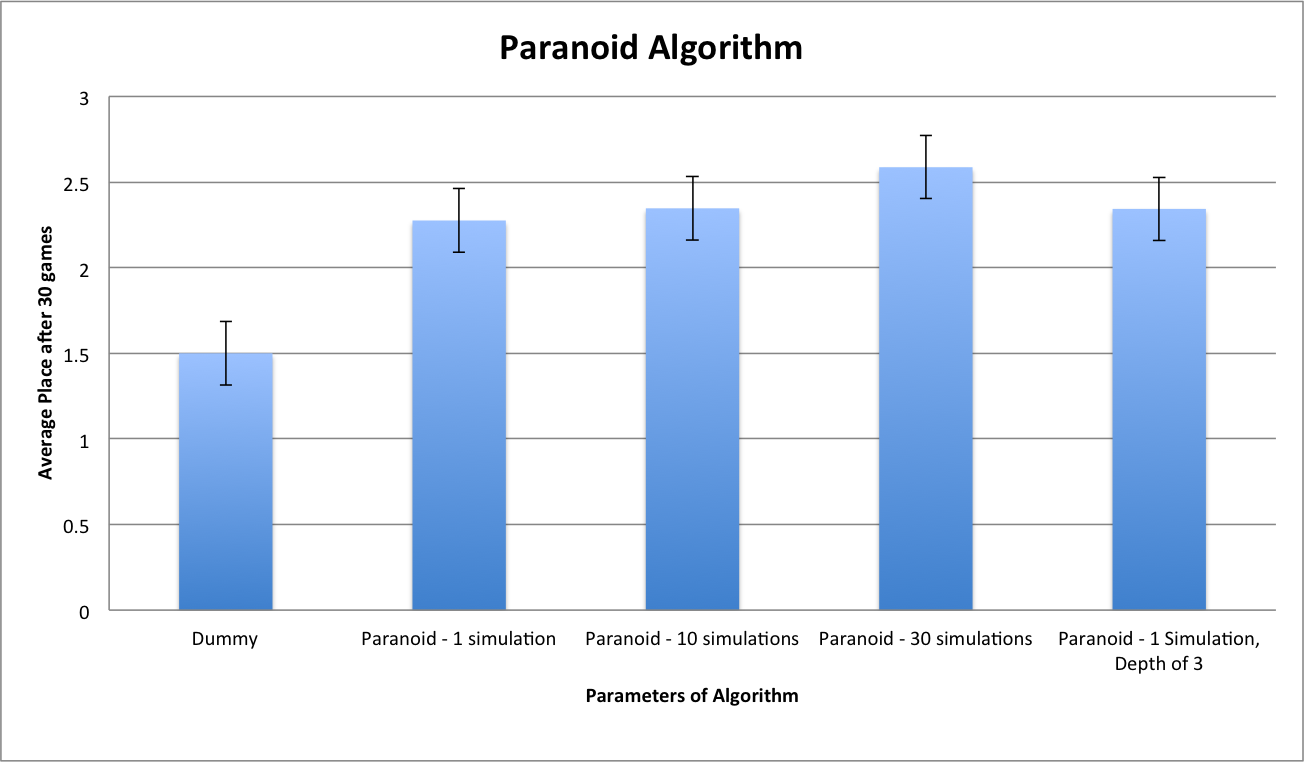
\includegraphics[width=\textwidth]{Paranoid.png}
\end{center}

We hypothesize that there are two main reasons that this happened.

\subsubsection{Monte Carlo Tree Search}

In the end, Monte Carlo Tree Search performed significantly worse than the baseline as seen in the following table:

\begin{center}
\textbf{MCTS Benchmark Results after 30 Simulations:}\\
\begin{tabular}{ c|c|c|c|c } 
 \hline

  & Number of Hands Sampled & Exploration Constant (c) & Budget (in s) & Score  (0-3)\\ 
\hline
 1 & 1 & 10 &  1 & 2.8\\ 
 2 & 1& 10 & .5 & 2.4 \\
3 & 1 & 1 & .5 & 2.5\\
4 & 10 & 10 & 1 & 2.66 \\
5 & 10 & 1 & 1  & 2.63 \\
 \hline
\end{tabular}
\end{center}
Even after altering the parameters for budget and exploration, the performance of the algorithm remained largely unchanged. In order to examine its shortcomings, we used the verbose option on the play game function to analyze its choice of actions in different scenarios. As it turns out, the MCTS agent consistently plays all its high cards first and is later forced to pass in the later stages of the game. The reason for this is that there is a dichotomy between its own actions and the actions it simulates in the tree. \\

When it expands a node and simulates a playout, it simulates itself playing as a dummy agent. Therefore, if a node corresponds to playing a 2 (meaning everyone else is forced to pass), it simulates from a state in which it has one card less than everyone else. In the simulation, it plays as a dummy agent meaning it gets rids of its lowest possible card all the time. In this scenario it makes sense for the MCTS agent it to play a high card to get 'ahead' and the play low the rest of the game as a dummy agent. However, the next time it is forced to play a card in the game it again picks a high card which runs contrary to what it simulated in the algorithm. In order to fix this, the simulation would have to play as itself and not as a dummy agent. However, this risks running into a circular definition of the algorithm and would involve huge computational costs as it would need to simulate itself repeatedly in order to choose a single action.\\

Given this analysis and the results of the simulations, we see that the poor performance of the algorithm is more due to inherent shortcomings of MCTS in its application to Presidents than from suboptimal choice of parameters. In order to improve the overall performance, a new approach is required.


 
\subsection{Discussion}
Overall, there are optimizations to be made in the approach to solving the constraint of imperfect information. As of now, the sampling of hands is done uniformly for each player. However, in the game of presidents, since the president and the asshole switch hands it is more likely that the asshole have a worse hand than the secretary, who didn't switch any cards, and that the secretary in turn have a worse hand than the president. This issue could be approached in several ways.\\

The first way would be to estimate the average hand strength of each respective player rank at each point in the game and then sample hands for that player based on that average. After playing a large number of games, we could infer the distribution for the hands of each depending on how many cards they have and then sample from that distribution. One major issue with this approach is that it is blind to past behavior of each agent. An agent could have been playing high cards all through the game and then be left with just low cards. However, the distribution for the player's hand at that point in the game could still be very high, giving the player an unrealistic set of cards.\\

 The second way to approach the problem would be to create a filtering algorithm that estimates the current hand strength based on the history of play of the player. Each card played would be considered an emission and the hidden states would be the player's hands after each time it plays. The trouble in this approach would be estimating the transition probabilities between hidden states as well as the emission probabilities for the played cards. Emissions are not independent of the top card on the deck. Also, it is not clear whether playing a high card means your next state is weaker or stronger. If for example, an agent plays a 2 and gets to go again (this is a rule of the game), he might: 1) have another 2 and a low card which menas he has the chance to win, or 2) he might be left with a 3 and be forced to pass for the next rounds.\\

In terms of improving MCTS, there is a lot of work that can be done refining the different parameter values. The performance of the algorithm is dependent on how well it selects nodes in the tree and then expands them. This exploration is regulated by means of a constant that can be altered. Moreover, the time budged can be changed to that it expands more of the tree. By optimizing the values for these two parameters, one can increase the efficiency of the algorithm and the quality of the actions taken. More importantly however, there are improvements to be made in the simulation of a playout from a node in order to remove the differences between actual and simulated games.\\

Lastly, we wrote a reinforcement learning agent for the game. However, we were unable to get it to work properly. Since the state space is so big (it depends on current, hand, top card, and the hands of every player), it was a challenge to condense the state space to a manageable size. Lastly, work is to be done tuning the parameters for the agent.

\section{References}

\begin{thebibliography}{5}

\bibitem{sturtevant03a}
	Sturtevant, Nathan.
	\emph{Comparison of Algorithms for MultiAgent Games.}
	Computers and Games.
	2003

\bibitem{browne12}
	Browne, Cameron.
	\emph{A Surver of Monte Carlo Tree Search Methods.}
	IIEEE Transactions on Computational Intelligence and AI in Games. 
	2012

\bibitem{fujita03}
	Fujita, Hajime.
	\emph{A reinforcement learning scheme for a multi-agent card game.}
	Systems, Man and Cybernetics.
	2003

\bibitem{kjeldsen01}
	Kjeldsen, Tinne Hoff.
	\emph{John von Neumann’s Conception of the Minimax Theorem: A Journey Through Different Mathematical Contexts}
	Arch. Hist. Exact Sci.
	2001
	
\bibitem{sturtevant03b}
	Sturtevant, Nathan.
	\emph{Multi-Player Games: Algorithms and Approaches.}
	2003
	
\bibitem{pfeffer95}
	Koller, Daphne, and Pfeffer, Avi.
	\emph{Generating and solving imperfect information games.}
	IJCAI.
	1995
	
\end{thebibliography}

\appendix

\section{Program Trace}



\section{System Description}

To actually implement our algorithms, we required a fairly in-depth and systematic description of the game itself. To do this, we created three main modules:
\begin{itemize}
  \item \textbf{state.py}. This module contains the State class, which we use to define and instantiate objects representing the state of the game. It contains many attributes relating to game state, such as which cards each player has played so far, the number of players in the game, whos turn it is, the current top card on the stack and who played it, and who has ran out of cards already (and in what order). It also keeps track of how many cards are remaining in each player's hand. This class provides many useful helper functions, such as \verb|getChild|, which provides the subsequent state given an action, and \verb|isFinalState|, which simply tells whether a state is terminal.
  \item \textbf{agent.py}. This module contains the Agent class, which is an abstract class to represent an agent in the game. The agent is given an ID and a hand at the beginning of the game, and then throughout the game the agent will be presented a State object and asked to make a move via the \verb|makeMove| function. This function is then overridden by each of the agents we wrote that inherit from Agent, each implementing their own algorithm in order to decide which move to make. The Agent class also provides helper functions, such as \verb|getAllActions|, which provides a list of legal actions given the agent's hand and the current state (passed in as an argument).
  \item \textbf{game.py}. This module contains the Game class, which we use to run and simulate games of Presidents. The Game class takes in, among other optional arguments, the agents for the game. Then, the game creates an initial state and goes around to each agent, calling their \verb|makeMove| function. Then, the game returns the order in which the players finished. There are also options within the Game class to run many repeated games; in these repeated games, the swapping of cards between the first- and worst-finishing agents (and second- and second-to-worst-finishing agents) occurs before each game.
\end{itemize}

 Appendix 2 – A clear description of how to use your system and how to generate the output you discussed in the write-up and the example transcript in Appendix 1. N.B.: The teaching staff must be able to run your system.

\section{Group Makeup}

\begin{itemize}
\item Matt Goldberg - Wrote the state, agent, and game modules that provide the necessary formalisms and rules to encode the game of Presidents. Also implemented the Max-N algorithm.
\item Nicholas Larus-Stone - Implemented the repeated games function that allows a list of agents to play multiple games. Implemented the Paranoid algorithm and the RL algorithm.

\item Juan Perdomo-  Implemented the formalisms necessary to implement the MCTS algorithm as well as implemented the algorithm itself.

All contributed equally to this writeup.
\end{itemize}


\end{document}
